\section{05. Mai 2015}

\question{Skizzieren Sie den Verlauf der Potentialkurve für ein homöopolares Molekül. Erklären Sie sie qualitativ.}
\label{q:11}

(Siehe auch \aqref{2}.)

Homöopolare Moleküle sind Moleküle, die aus Atomen desselben Elements bestehen. Sie entstehen durch kovalente Bindungen. In Abbildung \ref{fig:Frage_11} ist die Potentialkurve einer kovalenten Bindung dargestellt, welche mit einem Lennard-Jones-Potential angenähert werden kann. Für kleine Abstände dominiert der Faktor $\frac{a}{R^12}$ (Abstoßung der Elektronen durch Pauli-Prinzip) bei größeren Abständen der Faktor $-\frac{b}{R^6}$ (Van der Waals). Die Bindungsenergie $E_B$ befindet sich beim globalen Minimum. 
\begin{figure}[H]
    \centering
    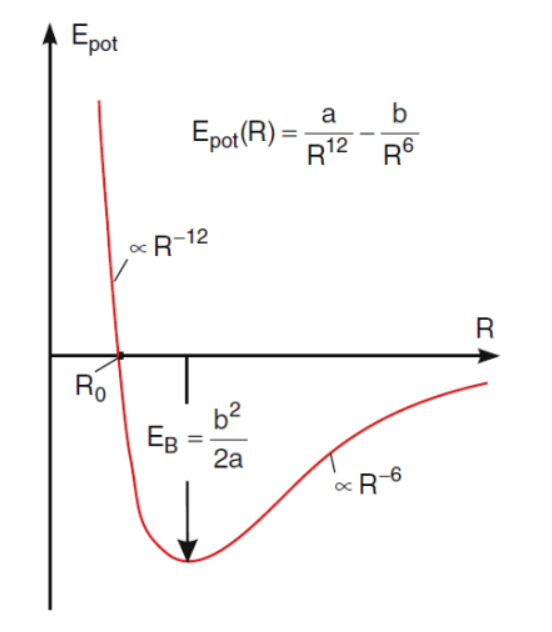
\includegraphics[width = 0.4\textwidth]{resources/05-05-2015/Frage_11.png}
    \caption{Potentialkurve homöopolare Molekül}
    \label{fig:Frage_11}
\end{figure}


\question{Erklären Sie die Herkunft der 'Austauschenergie' in H2. Wann ist sie groß, wann klein? Warum ist sie entscheidend für die chemische Bindung?}
\label{q:12}

Siehe \aqref{1}

\question{Welche Informationen über molekulare Kenngrößen können aus Rotations-Schwingungsspektren von Molekülen erhalten werden?}
\label{q:13}

Es können folgende Kenngrößen bestimmt werden:
\begin{itemize}
    \item Gleichgewichtsabstand $R_e$
    \item Rotationskonstanten $B_e$ und $\alpha_e$
    \item Form der Potentialkurve
\end{itemize}

\question{Diskutiere einen elektronischen Übergang in einem 2-Atomigen Molekül und die daraus resultierenden Schwingungsbanden im Spektrum.}
\label{q:14}

(Siehe auch \aqref{3}.)

Ändert sich die Schwingungsquantenzahl $\nu$ so ändert sich die Energie $E_{vib}$, bei Änderung der Rotationsquantenzahl $J$ die Energie $E_{rot}$ Die Gesamternergie setzt sich aus der Schwingungs- Rotations- und Potentiellenenergie zusammen:
\begin{equation}
    E = E_{rot} + E_{vib} + E_{pot}
\end{equation}
Der Abstand zwischen den einzelnen Energien $E_{rot}$ ist dabei deutlich kleiner als der zwischen den einzelnen Energien $E_{vib}$.\\
Übergänge zwischen Schwingungsrotationsniveaus $(\nu_i, J_i) \longleftrightarrow (\nu_k, J_k), \nu_i \neq \nu_k$: Schwingungsrotationsspektrum im infraroten Spektralbereich (\SIrange{2}{10}{\micro\meter})\\
Übergänge zwischen Schwingungsrotationsniveaus $(\nu_i, J_i) \longleftrightarrow (\nu_k, J_k), \nu_i = \nu_k$: Reines Rotationsspektrum, Mikrowellenbereich (\SIrange{e3}{e4}{\micro\meter})
\begin{figure}[H]
    \centering
    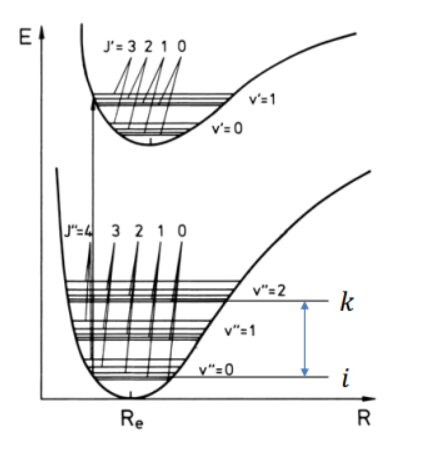
\includegraphics{resources/05-05-2015/Frage_14.png}
\caption{Übergänge zwischen Schwingungsrotationsniveaus}
    \label{fig:enter-label2}
\end{figure}

\question{Diskutiere den Zusammenhang zwischen Gitterebene im Kristall und Vektoren des reziproken Gitters.}
\label{q:15}

Siehe \aqref{4}.

\question{Diskutieren Sie die Wärmekapazität des Gitters im Rahmen des klassischen und der Quantenmechanik.}
\label{q:16}

%TODO: Bissl mehr Details

\textbf{Klassische Mechanik:}
\begin{itemize}
    \item Keine Translations- und Rotationsfreiheitsgrade
    \item Jedes Atom kann in 3 voneinander unabhängigen Raumrichtungen schwingen:
    \begin{itemize}
        \item 3 Schwingungsfreiheitsgrade der kinetischen Energie
        \item 3 Schwingungsfreiheitsgrade der potentiellen Energie
    \end{itemize}
\end{itemize}
Gesetzt von Dulong-Petit:
\begin{equation}
    f = 6 \qquad c_\nu^m = 3N_Ak_B = 3R = \SI{24.9}{\joule\per\mole\per\kelvin}
\end{equation}

\textbf{Quantenmechanik}
Quantisierung der Gitterschwingungen entscheidend für die innere Energie und
die spezifische Wärme des Kristallgitters.\\
Bei niedrigen Temperaturen ($k_BT \ll \hbar\omega$) kommt es zu einem Ausfrieren der Schwingungsfreiheitsgrade:
\begin{equation}
    c_\nu^m \rightarrow 0
\end{equation}
Bei hohen Temperaturen ($k_BT \gg \hbar\omega$):
\begin{equation}
    c_\nu^m \rightarrow 3R \qquad \text{gleich wie beim Gesetzt von Dulong-Petit}
\end{equation}


\question{Wie ermittelt man experimentell eine Phononendispersionskurve?}
\label{q:17}

Durch Streuung von Photonen, Neutronen oder Elektronen am Kristallgitter. 

\begin{figure}[H]
    \centering
    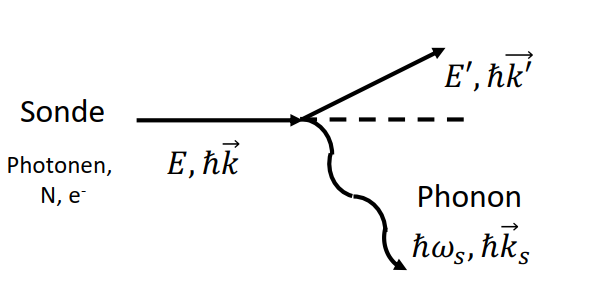
\includegraphics{resources/05-05-2015/Frage_17.png}
    \caption{Inelastische  Streuung an Phononen}
    \label{fig:enter-label}
\end{figure}
Die Dispersionsrelation ergibt sich dann zu:
\begin{equation}
    \omega_s(\vec{k_s})=\omega_s(\vec{k'}-\vec{k})
\end{equation}
Am besten durch Streuung von Neutronen: 
\begin{itemize}
    \item Energie und Impuls von Neutronen im selben Bereich wie Phononen
    \item Neutronen werden nur an Atomkernen gestreut und regen Gitterschwingungen an
\end{itemize}


\question{Erklären Sie das Zustandekommen von Energiebändern in Festkörper im Rahmen der Theorie der fast-freien Elektronen.}
\label{q:18}

Siehe \aqref{5}.

\question{Erklären Sie das Bloch'sche Theorem für Elektronen im periodischen Potential.}
\label{q:19}

Siehe \aqref{8}.

\question{Diskutieren Sie den Paulschen Paramagnetismus.}
\label{q:20}

\newpage
